% !TeX spellcheck = en_US
% !TeX encoding = UTF-8
\chapter*{Appendix}

\section{Code and files}

\begin{lstlisting}[style=text, caption={The DOT file of uncompressed block memgraph, here \textit{Training/basic/V\_7\_1\_P1/24/17016-1643962152-heap.raw}, with real addresses. Output is cropped.}, label={appendix:dot:17016-1643962152:cropped}]
    strict digraph "17016-1643962152" {
        "CHN(0x558343d21d40)" [label="CHN(1)" color="cyan" style=filled shape=square];
        "CHN(0x558343d1a448)" [label="CHN(2)" color="cyan" style=filled shape=square];
        "VN(0x558343d1a450)" [label="VN" color="grey" style=filled];
        "VN(0x558343d1a458)" [label="VN" color="grey" style=filled];
        "PN(0x558343d24ae8)" [label="PN" color="orange" style=filled shape=hexagon];
        "KN_KEY_A(0x558343d29460)" [label="KN(A)" color="green" style=filled];
        "KN_KEY_B(0x558343d2b960)" [label="KN(B)" color="green" style=filled];
        "CHN(0x558343d21d40)" -> "KN_KEY_A(0x558343d29460)" [label="dts" weight=1]
        "PN(0x558343d204e8)" -> "KN_KEY_A(0x558343d29460)" [label="ptr" weight=1]
        "CHN(0x558343d21d40)" -> "KN_KEY_B(0x558343d2b960)" [label="dts" weight=1]
        "PN(0x558343d2deb8)" -> "KN_KEY_B(0x558343d2b960)" [label="ptr" weight=1]
        "CHN(0x558343d21d40)" -> "KN_KEY_C(0x558343d29080)" [label="dts" weight=1]
        "PN(0x558343d204e0)" -> "KN_KEY_C(0x558343d29080)" [label="ptr" weight=1]
        "PN(0x558343d24ae8)" -> "VN(0x558343d1a010)" [label="ptr" weight=1]
        "PN(0x558343d1a240)" -> "VN(0x558343d20680)" [label="ptr" weight=1]
    }
\end{lstlisting}

\section{Memory Graphs}

\begin{figure}[H]\label{appendix:mem_graph:302-1644391327:full}
    \centering
    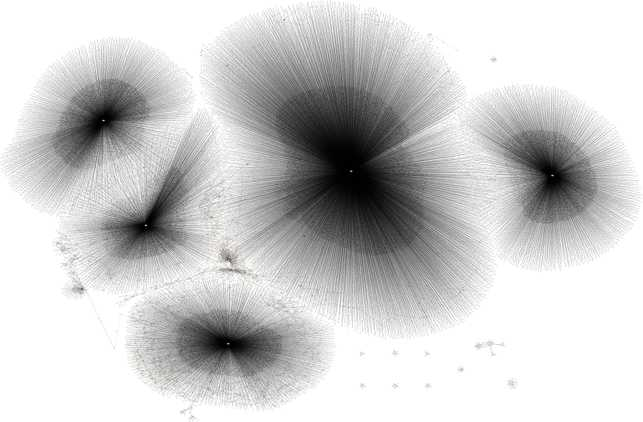
\includegraphics[width=16cm]{graphs/test_graph_from_302-1644391327_vn-sfdp.png}
    \caption{Visualization of the full memory graph generated from \textit{Training/scp/V\_7\_8\_P1/16/302-1644391327-heap.raw}.}
\end{figure}

\begin{figure}[H]\label{appendix:mem_graph:17016-1643962152:full}
    \centering
    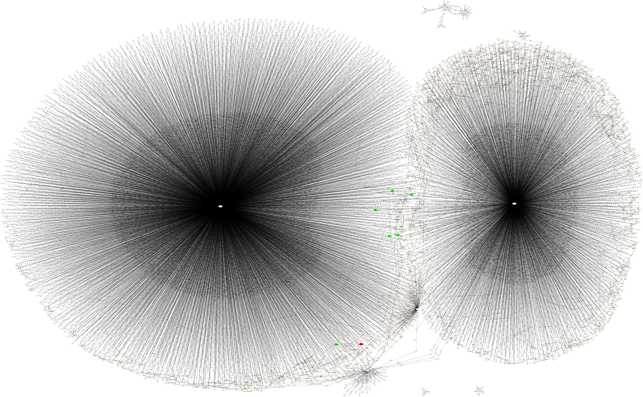
\includegraphics[width=16cm]{graphs/Training_basic_V_7_1_P1_24_17016-1643962152-heap.raw_dot_vn-sfdp.png}
    \caption{Visualization of the full memory graph generated from \textit{Training/basic/V\_7\_1\_P1/24/17016-1643962152-heap.raw}.}
\end{figure}

\begin{figure}[H]\label{appendix:mem_graph:17016-1643962152:truncated}
    \centering
    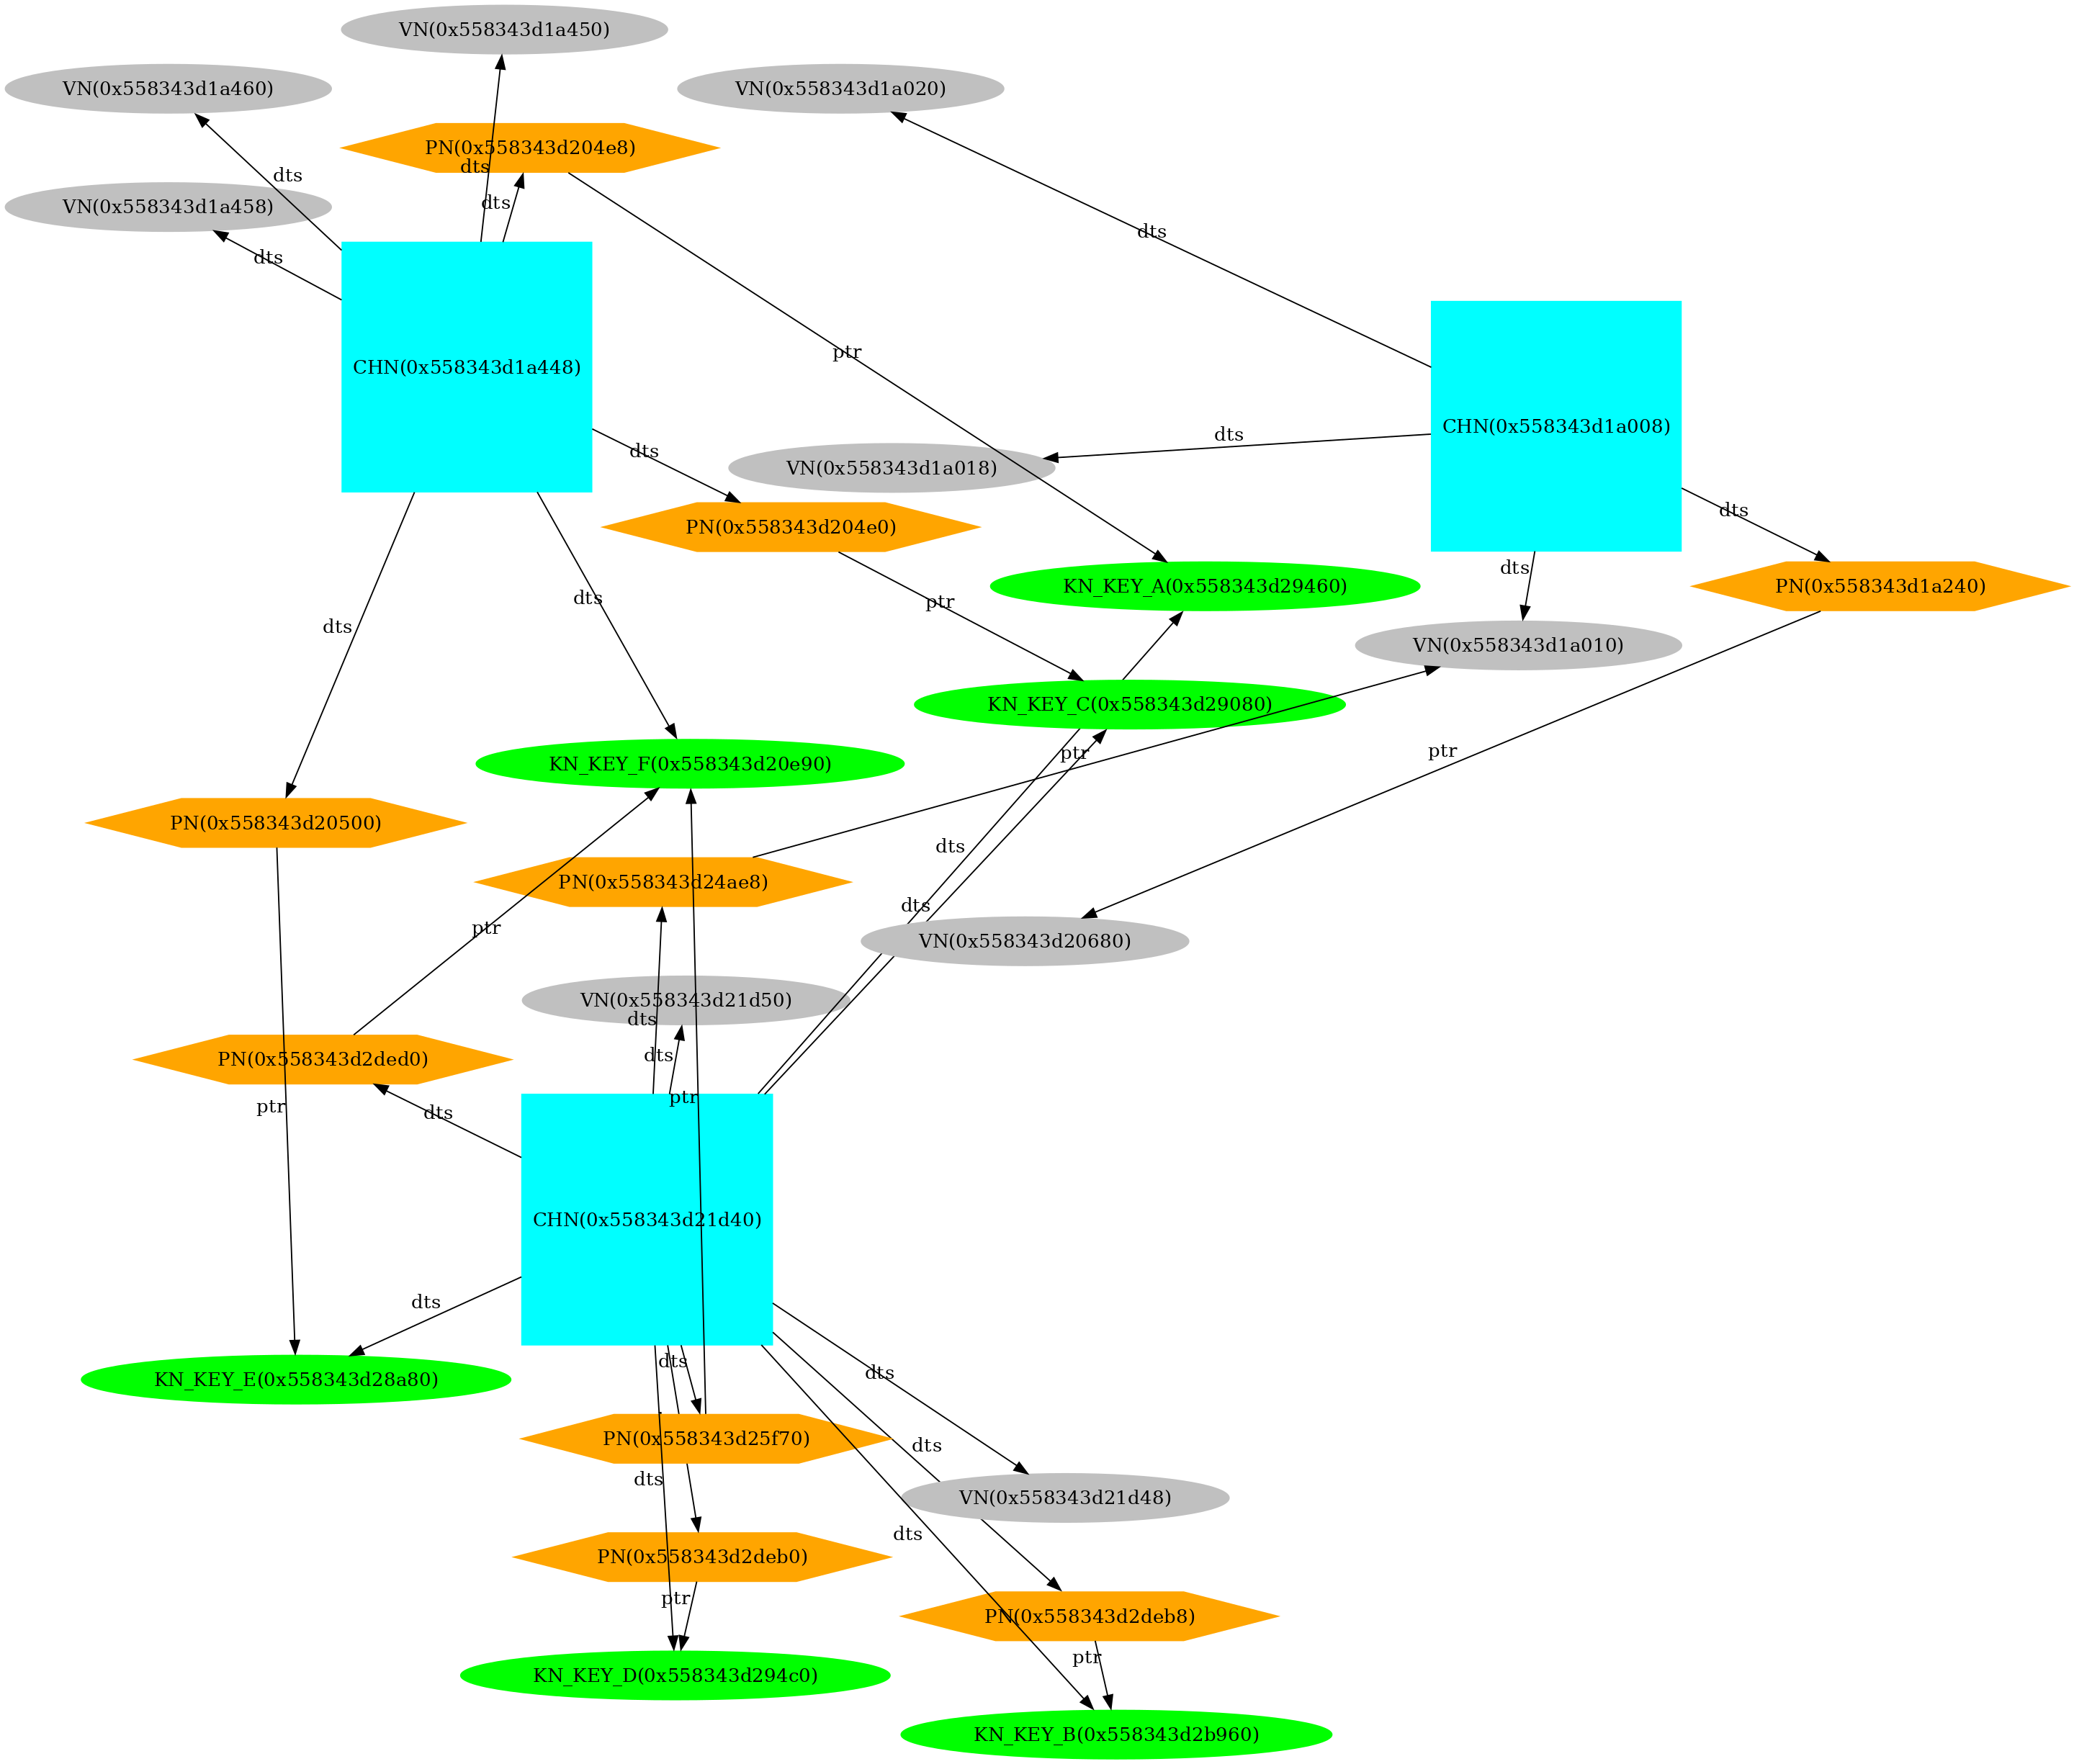
\includegraphics[width=16cm]{graphs/17016-1643962152_truncated.png}
    \caption{Visualization of a truncated memory graph generated from \textit{Training/basic/V\_7\_1\_P1/24/17016-1643962152-heap.raw}. Here with real addresses.}
\end{figure}

Generated using a slightly different command, for better layout of the nodes:

\begin{lstlisting}[language=bash, caption={Command used to generate the memory graph visualization of \textit{Training/basic/V\_7\_1\_P1/24/17016-1643962152-heap.raw} here using real addresses.}]
    sfdp -Gsize=30! -Goverlap=ortho -Tpng 17016-1643962152_truncated.gv > 17016-1643962152_truncated.png
\end{lstlisting}

\begin{figure}[H]
    \centering
    \includegraphics[width=16cm]{graphs/chunk_top_vn_semantic_home_onyr_code_phdtrack_phdtrack_data_clean_8708-1643979488-heap.raw_dot_no_vn_chn_annotation_no_vn-sfdp.png}
    \caption{Visualization of a chunk memory graph generated from \textit{Validation/Validation/basic/V\_7\_8\_P1/24/8708-1643979488-heap.raw}.}
\end{figure}

\begin{figure}[H]
    \centering
    \includegraphics[width=16cm]{graphs/chunk_top_vn_semantic_home_onyr_code_phdtrack_phdtrack_data_clean_28621-1643890740-heap.raw_dot_no_vn_chn_annotation_no_vn-sfdp.png}
    \caption{Visualization of a chunk memory graph generated from \textit{Training/Training/basic/V\_6\_8\_P1/24/28621-1643890740-heap.raw}.}
\end{figure}